\documentclass[a4paper,11pt]{article}
\usepackage[left=2.5cm,right=2.5cm,top=2.5cm]{geometry}
\usepackage[czech,slovak,english]{babel}
\usepackage[utf8]{inputenc}
\usepackage{url}
\usepackage{graphicx}
\usepackage{picture}
\usepackage{courier}
\usepackage{listings}

\addto\captionsenglish{\renewcommand{\figurename}{Obr.}}

\begin{document}

\section{Enumeration Sort}
Enumeration sort je je radiaci algoritmus, ktorý vzájomným porovnávaním všetkých prvkov nájde ich zoradenú postupnosť. V tomto prípade sa jedná o variantu pracujúcu nad lineárnym poľom N procesorov doplnených o spoločnú zbernicu a schopných preniesť jednu hodnotu v každom kroku. Počet procesorov odpovedá počtu radených prvkov. Nevýhodou tejto varianty algoritmu je, že nedokáže zoradiť radu obsahujúcu duplicitné prvky.

Ak na vstupe máme radu $X=(x_1, x_2, ..., x_n)$, potom každý procesor $i \in <1,N>$ pozostáva zo 4 registrov, ktoré obsahujú:
\begin{itemize}
\item $X_i$ prvok $x_i$ zo vstupnej rady
\item $Y_i$ postupne prvky $x_1$..$x_n$
\item $C_i$ koľkokrát platilo $X_i > Y_i$
\item $Z_i$ zoradený prvok $Y_i$
\end{itemize}

\subsection{Algoritmus}
\begin{enumerate}
\item Všetky registre C sa nastavia na hodnotu 1
\item 2n-krát opakuj ($ 1 \leq k \leq 2n$):
\begin{itemize}
\item Ak nie je vstup vyčerpaný, vstupný prvok $x_i$ sa vloží prostredníctvom zbernice do $X_i$ a lineárnym spojením sa obsah všetkých registrov $Y$ posunie doprava a do $Y_1$ sa vloží prvok $x_i$
\item Každý procesor $p$ s neprázdnymi registrami $X_p$ a $Y_p$ ich porovná a v prípade, ak $X_p > Y_p$ inkrementuje register $C_p$
\item Ak $k > n$, procesor $P_{k-n}$ pošle obsah svojho registru $X$ procesoru $P_{C_{k-1}}$, ktorý si túto hodnotu uloží do registru $Z$
\end{itemize}
\item V nasledujúcich n cykloch procesory posúvajú obsah svojich registrov Z doprava a procesor $P_n$ produkuje zoradenú postupnosť.
\end{enumerate}

\subsection{Zložitosť}
Predpokladajme, že prenos hodnoty zbernicou trvá konštantnú dobu nezávisle od fyzickej vzdialenosti procesorov. Potom krok 1 trvá konštantnú dobu, krok 2 trvá 2n cyklov a 3. krok trvá n cyklov. Dokopy teda:
\begin{itemize}
\item $ t(n) = O(n) $
\item $ p(n) = n $
\item $ c(n) = t(n) \cdot p(n) = O(n)\cdot n = O(n^2) $
\end{itemize}
Cena algoritmu nie je optimálna. Optimálna cena by bola $ c(n) = O(n \cdot \log n) $.

\section{Vlastná implementácia algoritmu}
Výsledná implementácia sa od uvedeného algoritmu mierne líši. Hlavným dôvodom je potreba zaistiť aj radenie radov s duplicitnými prvkami a využitie prvého procesora (master) ako riadiacej jednotky činnosti ostatných procesorov (slave). K tomuto účelu sú slave procesory doplnené o registre $ix$ a $iy$, v ktorých si ukladajú index hodnoty uloženej v príslušnom registry ($X$ alebo $Y$). Index hodnoty odpovedá ich poradiu vo vstupnej rade. Algoritmus je nasledovný:
\begin{enumerate}
\item Všetky registre C sa nastavia na hodnotu 1
\item Master procesor i-temu slave procesoru pošle $x_i$ spolu s indexom $i$ a procesor si ich uloží do registrov $X$ a $ix$. V rovnakom cykle postupne zasiela prvému slave procesoru tie isté hodnoty a ten si ich postupne ukladá do registrov $Y$ a $iy$
\item Slave procesory postupne porovnávajú hodnotu v registry $X$ s hodnotami v registry $Y$, ak platí $X > Y$ alebo $X = Y \wedge ix > iy$, tak inkrementuje obsah C registru
\item Ak má slave procesor následníka, zašle mu aktuálne hodnoty registrov $Y$ a $iy$.
\item Každý slave procesor zašle hodnotu registru X slave procesoru s číslom odpovedajúcemu hodnote C registru, cieľový procesor si ju uloží do registru Z
\item Slave procesory $p_i$ zašlú obsah Z registru master procesoru, ten ich prijme v poradí $i = 1..n$, a tým vyprodukuje výslednú postupnosť
\end{enumerate}

Komunikácia procesorov je znázornená na nasledovnom sekvenčnom diagrame. Zasielané správy v sekvenčnom diagrame majú formát \texttt{data, dest\_reg}, kde \texttt{data} sú zasielané hodnoty a \texttt{dest\_reg} cieľové registre prijímajúceho procesoru. Zátvorky [ ] značia pole hodnôt, prípadne index hodnoty v rade.

\begin{figure}[!htb]
\centering
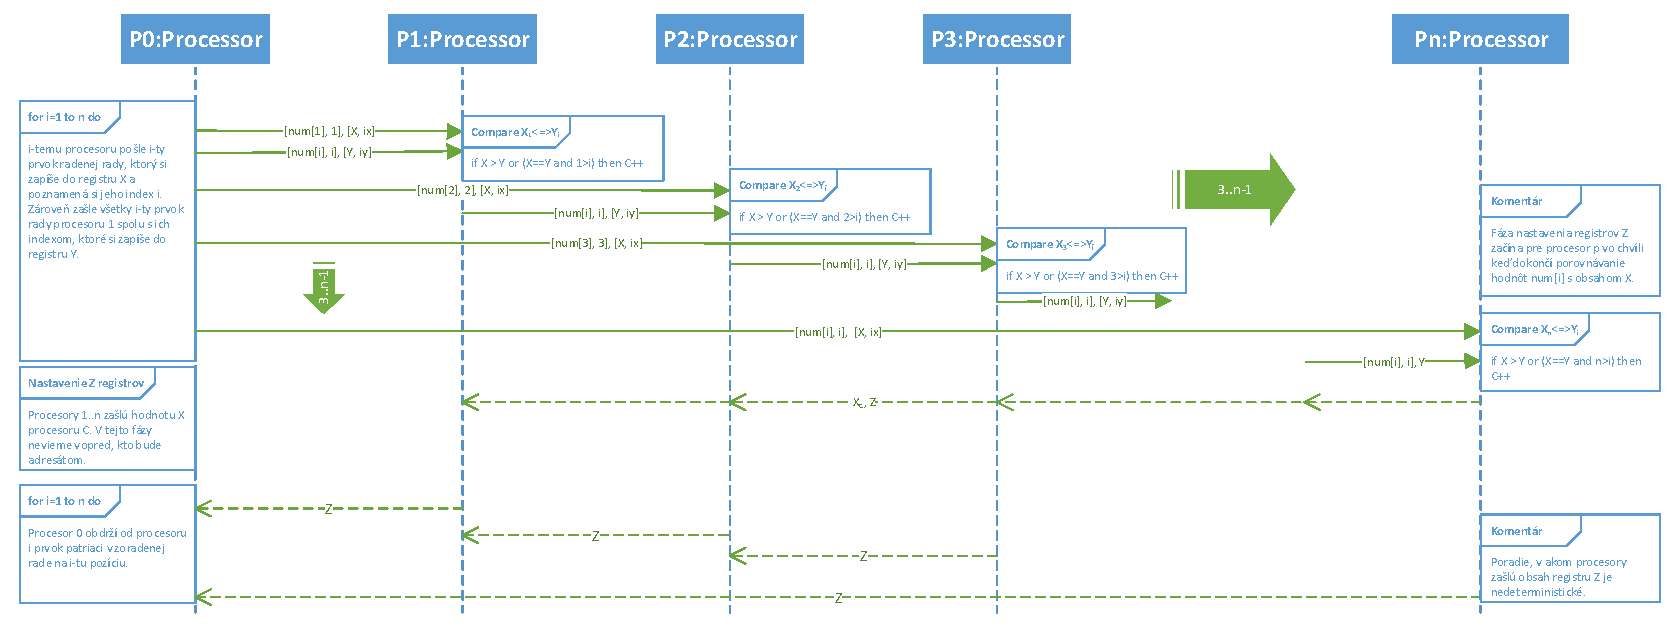
\includegraphics[width=\textwidth]{sequence.pdf}
\caption{Sekvenčný diagram}
\end{figure}

\subsection{Namerané hodnoty}
Na meranie času bola použitá funkcia \texttt{std::chrono::high\_resolution\_clock::now()} zo štandardnej knižnice C++ \texttt{chrono}, preto je program nutné prekladať s parametrom \texttt{--std=C++11}. Meranie pre každú veľkosť vstupných dát bolo vykonané 10x. Vzhľadom na to, že sa nepodarilo ani po zvýšení limitov spustiť program s viac ako 32 procesormi, je najväčší vstup 30B. Namerané priemerné hodnoty pre rôzne veľkosti vstupu sú zobrazené na nasledujúcom grafe:

\begin{figure}[!htb]
\centering
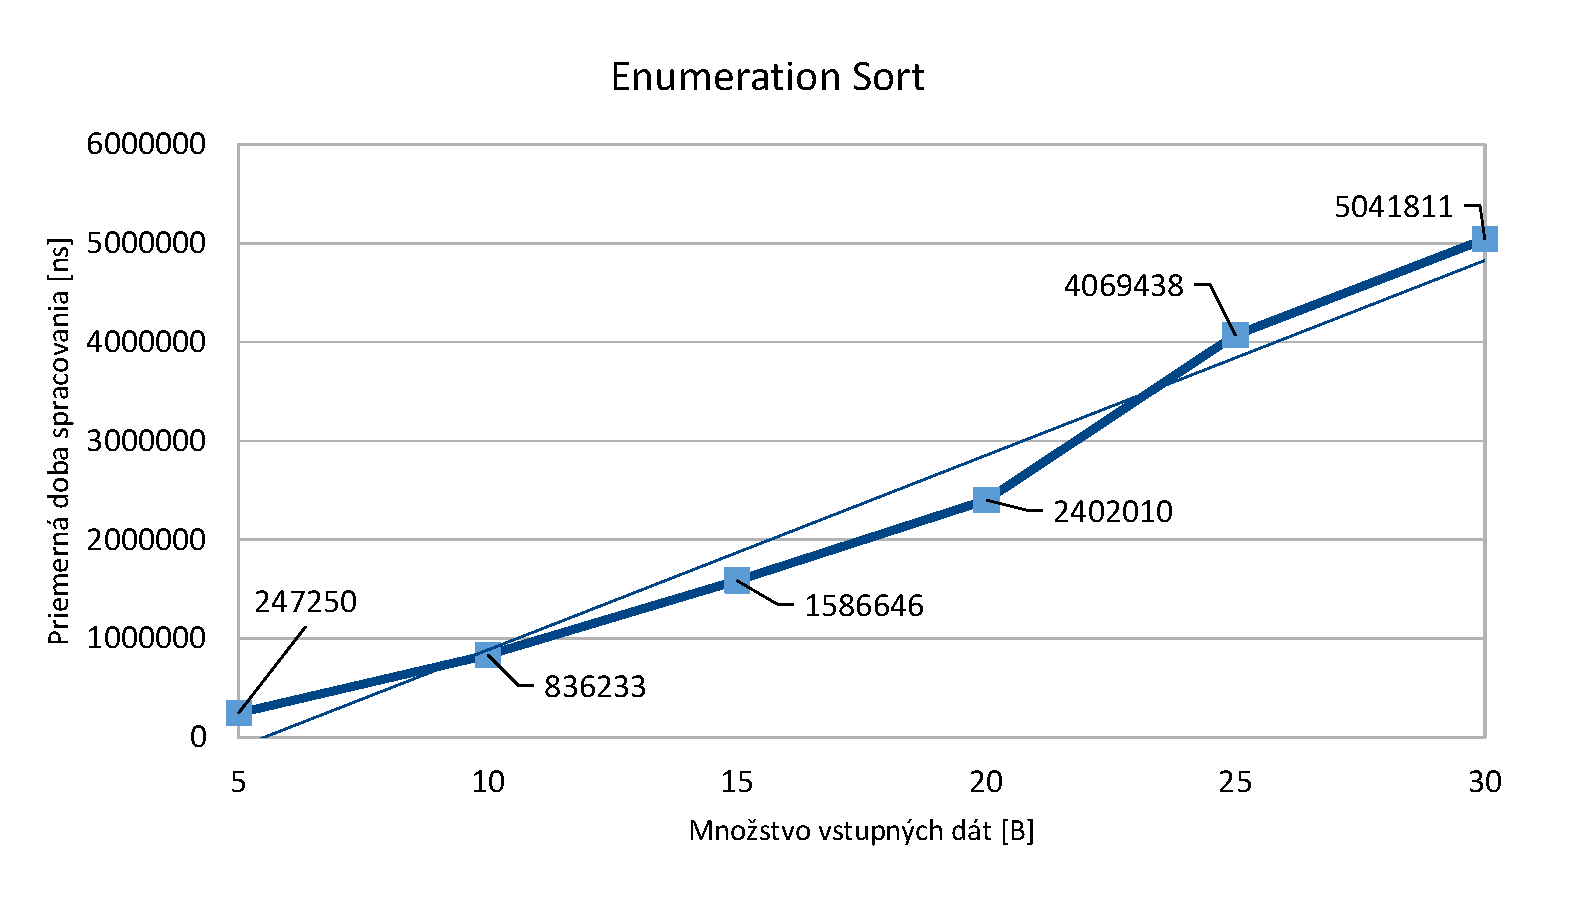
\includegraphics[width=\textwidth]{stats.pdf}
\caption{Namerané časy}
\end{figure}

\section{Záver}
Z nameraných hodnôt znázornených v grafe možno vyvodiť, že implementovaný algoritmus dodržuje teoretickú zložitosť algoritmu. Krivka s menšími odchýlkami kopíruje trendovú úsečku. Odchýlky sú spôsobené rozdielmi medzi jednotlivými meraniami, kedy niektoré namerané hodnoty sa líšili takmer dvojnásobne. Zvýšením počtu meraní by sa dosiahli presnejšie výsledky.
Implementovaný algoritmus by bolo možné zjednodušiť odstránením kroku 5 a namiesto toho by slave procesory posielali master procesoru dvojicu hodnôt - X a C. Ten by hodnoty umiestnil na správny index a následne vyprodukoval výslednú postupnosť.

\end{document}
